\documentclass[a4paper, 12pt]{article}		% general format

%%%% Charset
\usepackage{cmap}							% make PDF files searchable and copyable
\usepackage[utf8x]{inputenc} 				% accept different input encodings
\usepackage[T2A]{fontenc}					% russian font
\usepackage[russian]{babel}					% multilingual support (T2A)

%%%% Graphics
\usepackage[dvipsnames]{xcolor}			% driver-independent color extensions
\usepackage{graphicx}						% enhanced support for graphics
\usepackage{wrapfig}						% produces figures which text can flow around

%%%% Math
\usepackage{amsmath}						% American Mathematical Society (AMS) math facilities
\usepackage{amsfonts}						% fonts from the AMS
\usepackage{amssymb}						% additional math symbols

%%%% Typograpy (don't forget about cm-super)
\usepackage{microtype}						% subliminal refinements towards typographical perfection
\linespread{1.3}							% line spacing
\usepackage[left=2.5cm, right=1.5cm, top=2.5cm, bottom=2.5cm]{geometry}
\setlength{\parindent}{0pt}					% we don't want any paragraph indentation
\usepackage{parskip}						% not big distance between paragraphs

%%%% Tables
\usepackage{tabularx}						% Normal tables
\usepackage{multirow}						% for tabular
\usepackage{hhline}							% for tabular

%%%% Graph
\usepackage{tikz}
\usetikzlibrary{arrows}

%%%% Other
\usepackage{url}							% verbatim with URL-sensitive line breaks
\usepackage{fancyvrb}						% verbatim with box
%------------------------------------------------------------------------------
\usepackage{listings}						% typeset source code listings

% Цвета для кода
\definecolor{mygreen}{HTML}{3F7F5F} 		% color values Red, Green, Blue
\definecolor{mylilas}{RGB}{170,55,241}

% Настройки отображения кода
\lstset{language=Matlab,%
    %basicstyle=\color{red},
    breaklines=true,						% Перенос длинных строк
    morekeywords={matlab2tikz},
    keywordstyle=\color{blue},%
    morekeywords=[2]{1}, keywordstyle=[2]{\color{black}},
    identifierstyle=\color{black},%
    stringstyle=\color{mylilas},
    commentstyle=\color{mygreen},%
    showstringspaces=false,					% don't mark spaces in strings
    frame=tblr								% draw a frame at all sides of the code block
	rulecolor=\color{frame},				% Цвет рамки
	tabsize=2,								% tab space width
	showstringspaces=false,					% don't mark spaces in strings
    numbers=left,%
    numberstyle={\tiny \color{black}},% size of the numbers
    numbersep=9pt, % this defines how far the numbers are from the text
    emph=[1]{for,end,break},emphstyle=[1]\color{red}, %some words to emphasise
    %emph=[2]{word1,word2}, emphstyle=[2]{style},    
	% Для отображения русского языка
	extendedchars=true,
	literate={Ö}{{\"O}}1
	 	{Ä}{{\"A}}1
	 	{Ü}{{\"U}}1
		{ß}{{\ss}}1
		{ü}{{\"u}}1
		{ä}{{\"a}}1
		{ö}{{\"o}}1
		{~}{{\textasciitilde}}1
		{а}{{\selectfont\char224}}1
		{б}{{\selectfont\char225}}1
		{в}{{\selectfont\char226}}1
		{г}{{\selectfont\char227}}1
		{д}{{\selectfont\char228}}1
		{е}{{\selectfont\char229}}1
		{ё}{{\"e}}1
		{ж}{{\selectfont\char230}}1
		{з}{{\selectfont\char231}}1
		{и}{{\selectfont\char232}}1
		{й}{{\selectfont\char233}}1
		{к}{{\selectfont\char234}}1
		{л}{{\selectfont\char235}}1
		{м}{{\selectfont\char236}}1
		{н}{{\selectfont\char237}}1
		{о}{{\selectfont\char238}}1
		{п}{{\selectfont\char239}}1
		{р}{{\selectfont\char240}}1
		{с}{{\selectfont\char241}}1
		{т}{{\selectfont\char242}}1
		{у}{{\selectfont\char243}}1
		{ф}{{\selectfont\char244}}1
		{х}{{\selectfont\char245}}1
		{ц}{{\selectfont\char246}}1
		{ч}{{\selectfont\char247}}1
		{ш}{{\selectfont\char248}}1
		{щ}{{\selectfont\char249}}1
		{ъ}{{\selectfont\char250}}1
		{ы}{{\selectfont\char251}}1
		{ь}{{\selectfont\char252}}1
		{э}{{\selectfont\char253}}1
		{ю}{{\selectfont\char254}}1
		{я}{{\selectfont\char255}}1
		{А}{{\selectfont\char192}}1
		{Б}{{\selectfont\char193}}1
		{В}{{\selectfont\char194}}1
		{Г}{{\selectfont\char195}}1
		{Д}{{\selectfont\char196}}1
		{Е}{{\selectfont\char197}}1
		{Ё}{{\"E}}1
		{Ж}{{\selectfont\char198}}1
		{З}{{\selectfont\char199}}1
		{И}{{\selectfont\char200}}1
		{Й}{{\selectfont\char201}}1
		{К}{{\selectfont\char202}}1
		{Л}{{\selectfont\char203}}1
		{М}{{\selectfont\char204}}1
		{Н}{{\selectfont\char205}}1
		{О}{{\selectfont\char206}}1
		{П}{{\selectfont\char207}}1
		{Р}{{\selectfont\char208}}1
		{С}{{\selectfont\char209}}1
		{Т}{{\selectfont\char210}}1
		{У}{{\selectfont\char211}}1
		{Ф}{{\selectfont\char212}}1
		{Х}{{\selectfont\char213}}1
		{Ц}{{\selectfont\char214}}1
		{Ч}{{\selectfont\char215}}1
		{Ш}{{\selectfont\char216}}1
		{Щ}{{\selectfont\char217}}1
		{Ъ}{{\selectfont\char218}}1
		{Ы}{{\selectfont\char219}}1
		{Ь}{{\selectfont\char220}}1
		{Э}{{\selectfont\char221}}1
		{Ю}{{\selectfont\char222}}1
		{Я}{{\selectfont\char223}}1
		{і}{{\selectfont\char105}}1
		{ї}{{\selectfont\char168}}1
		{є}{{\selectfont\char185}}1
		{ґ}{{\selectfont\char160}}1
		{І}{{\selectfont\char73}}1
		{Ї}{{\selectfont\char136}}1
		{Є}{{\selectfont\char153}}1
		{Ґ}{{\selectfont\char128}}1
}

% Для настройки заголовка кода
\usepackage{caption}
\DeclareCaptionFont{white}{\color{сaptiontext}}
\DeclareCaptionFormat{listing}{\parbox{\linewidth}{\colorbox{сaptionbk}{\parbox{\linewidth}{#1#2#3}}\vskip-4pt}}
%\captionsetup[lstlisting]{format=listing,labelfont=white,textfont=white}
\renewcommand{\lstlistingname}{Листинг} % Переименование Listings в нужное именование структуры

%------------------------------------------------------------------------------

\begin{document}

\begin{titlepage}
\thispagestyle{empty}

\begin{center}
Санкт-Петербургский политехнический университет Петра Великого\\
Институт Информационных Технологий и Управления\\*
Кафедра компьютерных систем и программных технологий\\*
\hrulefill
\end{center}

\vspace{15em}

\begin{center}
\textsc{\textbf{Курсовая работа}}
\vspace{1em}

Дисциплина: \textbf{Методы оптимизации}
\vspace{2em}

Тема: \textbf{Формулировка и решение задачи выбора оптимального решения с использованием различных математических моделей}
\end{center}

\vspace{16em}

\begin{flushleft}
Выполнил студент гр. 53501/3 \hrulefill С.А. Мартынов \\
\vspace{1.5em}
Руководитель, к.т.н.,доц. \hrulefill А.Г. Сиднев\\
\end{flushleft}

\vspace{\fill}

\begin{center}
Санкт-Петербург \\
2015
\end{center}

\end{titlepage}
\setcounter{page}{2}
\tableofcontents

%------------------------------------------------------------------------------
%\section{Introduction.}

\par Currently, deep learning is an open-ended research area. With their success, deep learning is required to constantly increase the ability to go around data and relatively cheap graphics processors, allowing to build an effective calculation procedure.
In-depth training through sequential non-linear transformations, which, as a rule, are represented in the form of artificial neural networks. Today, they are used to solve such problems as prediction, pattern recognition and a number of others.
\par Deep learning is a subset of machine learning methods that use artificial neuron networks, built on the basis of an analogy with the structure of the neurons of the human brain. The term “deep” implies a large number of layers in the neural network.
\par Google, Microsoft, Amazon, Apple, Facebook and many other deep learning methods are used to analyze large data sets. Now this knowledge and skills went beyond purely academic research and became the property of large industrial companies.
\par The relevance of the topic of deep learning is confirmed by the regular appearance of articles on this topic.

\par The aim of the thesis is the development of teaching tools for the study of models of deep learning. In accordance with the purpose of the study, the following tasks were set:
\begin{itemize}
    \item analyze the main laboratory work;
    \item compare and choose technology for modeling deep neyron
networks;
    \item develop and test several laboratory works.
    \end{itemize}
\newpage
\section*{Введение}
\addcontentsline{toc}{section}{Введение}

В главе 3 рассматриваются марковские цепи, которые являются одним из основных инструментов моделирования стохастических систем. 

Существует два метода решения задачи с бесконечным числом этапов. Первый метод основан на переборе всех возможных стационарных стратегий в задаче при­нятия решений. Этот подход, по существу, эквивалентен методу полного перебора, и его можно использовать только тогда, когда общее число стационарных страте­гий с точки зрения практических вычислений достаточно мало. Второй метод, на­зываемый методом итераций по стратегиям, как правило, более эффективен, так как определяет оптимальную стратегию итерационным путем.
%------------------------------------------------------------------------------

\newpage
\section{Варианты формализации многокритериальной задачи и их решение с использованием Optimization Toolbox  системы Matlab.}


\subsection{Постановка задачи}
Мебельная  фабрика выпускает столы, стулья, бюро и книжные шкафы. При изготовлении используются два типа досок, причем фабрика имеет в наличии 1500 м досок первого типа и 1000 м досок второго типа. Кроме того, заданы трудовые ресурсы в количестве 800 чел/час. В таблице приводятся нормативы затрат каждого из видов ресурсов на изготовление 1 ед изделия и прибыль от реализации 1  ед  изделия.

\begin{table}[htb]
	\begin{tabularx}{\textwidth}{|X|c|c|c|c|}
	\hline 
	\multirow{2}{*}{Ресурсы} & \multicolumn{4}{c|}{Затраты на 1 ед изделия} \\ 
	\hhline{~----}
	{} & столы & стулья & бюро & Книжные шкафы \\ 
	\hline 
	Доски первого типа, м & 5 & 1 & 9 & 12 \\ 
	\hline 
	Доски второго типа, м & 2 & 3 & 4 & 1 \\ 
	\hline 
	Трудовые ресурсы, чел/час & 3 & 2 & 5 & 10 \\ 
	\hline 
	Прибыль, руб/шт & 12 & 5 & 15 & 10 \\ 
	\hline 
	\end{tabularx} 
\caption{Нормативы затрат ресурсов на единицу изделия}
\end{table}

По этим исходным данным решить задачу определения оптимальный ассортимент, максимизирующий прибыль (разность между выручкой и расходами.) и выручку при следующих ценах изготавливаемую мебель:

\begin{itemize}
\item стол -- 32 руб;
\item стул -- 15 руб;
\item бюро -- 12 руб;
\item книжный шкаф -- 80 руб.
\end{itemize}

В отчёте необходимо описать:
\begin{enumerate}
	\item Осуществление перехода от многокритериальной задачи к однокритериальной с использованием различных подходов.
	\item Решение задачи стохастического программирования для одной из однокритериальных задач, превратив детерминированное ограничение в вероятностное по схеме:
	$P(\sum\limits_{j=1}^n a_{ij}k_j-b_j\leq0)\geq\alpha_i$
	
	Менять $\alpha_i$ в следующем диапазоне $0.1 \leq \alpha_i \leq 0.9$.
	
	Считать случайной величиной $b_i$ или элементы $\{a_{ij}\}$ $i$-й строки матрицы $A$ $\{a_{ij}\}$ (по выбору).
\end{enumerate}

\subsection{Выделение главного критерия}
Выбирается один из критериев, например $C_i$, который наиболее полно отражает цель принятия решений. Остальные критерии учитываются только с точки зрения возможного указания их нижних границ $C_j(a) \geq \gamma_i$, $ j\neq i$. Таким образом, исходная задача многокритериального принятия решений заменяется однокритериальной задачей с критерием $C_i$, т.е. $a^* = \text{arg max } C_i(a)$, при ограничениях $C_k (a) \geq \gamma_i$, $k\neq i$.

Критерии:
\begin{itemize}
\item $max (12x_1+5x_2+15x_3+10x_4)$ (прибыль)
\item $max (32x_1+15x_2+12x_3+80x_4)$ (выручка)
\end{itemize}

Ограничения:
\begin{itemize}
\item $5x_1+x_2+9x_3+12x_4 \leq 1500$ (доски первого типа)
\item $2x_1+3x_2+4x_3+1x_4 \leq 1000$ (доски второго типа)
\item $3x_1+2x_2+5x_3+1x_4 \leq 800$ (трудовые ресурсы)
\end{itemize}

\subsubsection{Максимизация выручки}

Целевая функция:

$f = min (-32x_1-15x_2-12x_3-80x_4)$

Начальные условия:

$x_0 =
\begin{pmatrix}
  0 \\
  0 \\
  0 \\
  0
\end{pmatrix}$

Ограничения:

$A =
\begin{pmatrix}
  5 & 1 & 9 & 12 \\
  2 & 3 & 4 & 1 \\
  3 & 2 & 5 & 1 \\
  -1& 0 & 0 & 0 \\
  0 &-1 & 0 & 0 \\
  0 & 0 &-1 & 0 \\
  0 & 0 & 0 & -1
\end{pmatrix}$

$b =
\begin{pmatrix}
  1500 \\
  1000 \\
  800 \\
  0 \\
  0 \\
  0 \\
  0
\end{pmatrix}$

\lstinputlisting[language=Matlab, caption={Поиск оптимального решения для максимизация выручки}]{../task1/max_gain.m}

Результат:
\begin{itemize}
\item $x_1 = -0,0000$
\item $x_2 = 300,0000$
\item $x_3 = 0$
\item $x_4 = 100,0000$
\item $f1 = -2500$
\item $f2 = -12500$
\end{itemize}

\subsubsection{Максимизация прибыли}

Целевая функция:

$f = min (-12x_1-5x_2-15x_3-10x_4)$

Начальные условия:

$x_0 =
\begin{pmatrix}
  0 \\
  0 \\
  0 \\
  0
\end{pmatrix}$

Ограничения:

$A =
\begin{pmatrix}
  5 & 1 & 9 & 12 \\
  2 & 3 & 4 & 1 \\
  3 & 2 & 5 & 1 \\
  -1& 0 & 0 & 0 \\
  0 &-1 & 0 & 0 \\
  0 & 0 &-1 & 0 \\
  0 & 0 & 0 & -1 \\
  -32 & -15 & -12 & -80
\end{pmatrix}$

$b =
\begin{pmatrix}
  1500 \\
  1000 \\
  800 \\
  0 \\
  0 \\
  0 \\
  0 \\
  -12500
\end{pmatrix}$

\newpage
\lstinputlisting[language=Matlab, caption={Поиск оптимального решения для максимизация прибыли}]{../task1/max_profit.m}

Результат:
\begin{itemize}
\item $x_1 = 261,2903$
\item $x_2 = 0$
\item $x_3 = 0,0000$
\item $x_4 = 16,1290$
\item $f1 = -3296,8$
\item $f2 = -9651,6$
\end{itemize}

\subsection{Свертка критериев}

Максимизируется критерий объединенной операции, получающийся в результате суммирования всех частных критериев:

$C(a)=\sum\limits_{i=1}^m w_i C_i^n (a)$

$C_i^n (a)=\frac{C_i (a)}{C_i^*}$

$C_i^*$ - оптимальное решение задачи по каждому критерию в отдельности, $w_1+w_2+\dots+w_m=1$.

\lstinputlisting[language=Matlab, caption={Свертка критериев}]{../task1/convolution.m}

В fmincon передается сумма нормированных значений (первый критерий делится на f1, второй на f2), каждое из которых умножено на определенный весовой коэффициент. Результат:
\begin{itemize}
\item $x_1 = 166,4573$
\item $x_2 = 127,8185$
\item $x_3 = -0,0000$
\item $x_4 = 44,9913$
\item $f = -0,9019$ (суммарное)
\end{itemize}

\subsection{Максимин или минимакс}

Максиминную свертку представим в следующем виде: $C_i(a)= \text{min } w_i C_i(a)$

Решение $a^*$ является наилучшим, если для всех $a$ выполняется условие $C(a^*) \geq C(a)$, или $a^* = \text{arg max } C(a) = \text{arg max min } w_i C_i (a)$.

Решение задачи представлено как программа в среде Matlab, с использованием функции fminimax:

$f_1=((12x_1+5x_2+15x_3+10x_4)/3214)^{-1}$;

$f_2=((32x_1+15x_2+12x_3+80x_4 )^2/12500)^{-1}$;

\lstinputlisting[language=Matlab, caption={Содержание файла maxmin.m}]{../task1/maxmin.m}

\newpage
\lstinputlisting[language=Matlab, caption={Содержание файла funminmax.m}]{../task1/funminmax.m}

Так как в среде Matlab реализована только функция fminimax, которая минимизирует наихудшие значения системы функций нескольких переменных, начиная со стартовой оценки ($x_0$), то для реализации максиминной свертки необходимо в fminimax передавать функции, возведенные в степень "-1" (функция funminmax).

Результат:
\begin{itemize}
\item $x_1 = 111,6707$
\item $x_2 = 201,6612$
\item $x_3 = -0,0000$
\item $x_4 = 61,6654$
\item $f1 = 1,0840$
\item $f2 = 1,0840$
\end{itemize}

\subsection{Метод последовательных уступок}

Для решения данной задачи была выбрана уступка = 10\%. Решение задачи представлено как программа в среде Matlab, с использованием функции fmincon.

Целевые функции:
\begin{itemize}
\item $f_1=-(12x_1+5x_2+15x_3+10x_4)$
\item $f_2=-(32x_1+15x_2+12x_3+80x_4)$
\end{itemize}

Для первого критерия:

$A =
\begin{pmatrix}
  5 & 1 & 9 & 12 \\
  2 & 3 & 4 & 1 \\
  3 & 2 & 5 & 1 \\
  -1& 0 & 0 & 0 \\
  0 &-1 & 0 & 0 \\
  0 & 0 &-1 & 0 \\
  0 & 0 & 0 & -1
\end{pmatrix}$

$b =
\begin{pmatrix}
  1500 \\
  1000 \\
  800 \\
  0 \\
  0 \\
  0 \\
  0
\end{pmatrix}$

Результат:
\begin{itemize}
\item $x_1 = 261,29$
\item $x_2 = 0$
\item $x_3 = 0$
\item $x_4 = 16,13$
\item $f1 = 3297$
\item $f2 = 9651$
\end{itemize}

3297 – 329,7 = 2967,3  (10\%)

Для второго критерия:

$A =
\begin{pmatrix}
  5 & 1 & 9 & 12 \\
  2 & 3 & 4 & 1 \\
  3 & 2 & 5 & 1 \\
  -1& 0 & 0 & 0 \\
  0 &-1 & 0 & 0 \\
  0 & 0 &-1 & 0 \\
  0 & 0 & 0 & -1 \\
  -5 & -1 & -9 & -12
\end{pmatrix}$

$b =
\begin{pmatrix}
  1500 \\
  1000 \\
  800 \\
  0 \\
  0 \\
  0 \\
  0 \\
  -2967,3
\end{pmatrix}$

Результат:
\begin{itemize}
\item $x_1 = 112,7$
\item $x_2 = 200,3$
\item $x_3 = 0$
\item $x_4 = 61,4$
\item $f1 = 2967$
\item $f2 = 11519$
\end{itemize}

\subsection{Fgoalattain}

fgoalattain решает задачу достижения цели, которая является одной из формулировок задач для векторной оптимизации.

x = fgoalattain(fun, $x_0$, goal, weight):
\begin{itemize}
\item fun -- целевая функция, 
\item $х_0$ -- начальные значения,
\item goal -- целевые значения,
\item weight -- веса.
\end{itemize}

Решение задачи представлено как программа в среде Matlab, с использованием функций fminicon и fgoalattain.

Целевые значения:

Goal =(15855000 10240038400036 68000000 38080000 4900000) 

\newpage
Веса:

weight=abs(goal) -- для того, чтобы приближение к критериям было одинаково

\lstinputlisting[language=Matlab, caption={Содержание файла fgoalattain.m}]{../task1/fgoalattain.m}

Результат:
\begin{itemize}
\item $x_1 = 207,81$
\item $x_2 = 72,08$
\item $x_3 = 0$
\item $x_4 = 32,4$
\item $f1 = 3178$
\item $f2 = 10324$
\item $Att. = 0,1741$
\end{itemize}

\subsection{Задача стохастического программирования}

Требуется найти такие $x_1$, $x_2$, $x_3$, $x_4$ для которых выполняться следующие ограничения:
\begin{itemize}
\item $5x_1+x_2+9x_3+12x_4 \leq 1500$
\item $2x_1+3x_2+4x_3+1x_4 \leq 1000$
\item $3x_1+2x_2+5x_3+1x_4 \leq 800$
\end{itemize}

Перейдем от последнего ограничения к вероятностному по схеме:
$P(\sum\limits_{j=1}^n a_{ij}k_j-b_j\leq0)\geq\alpha_i$
	
И будем менять $\alpha_i$ в диапазоне $0.1 \leq \alpha_i \leq 0.9$, и возьмём коэффициенты $a_i$ за случайные величины.

$P(0,6x_1 + 0,8x_2 + 1,0x_3 + 1,2x_4 \leq 100) \geq \alpha_i$

Пользуясь формулой:
$\sum\limits_{j=1}^3 a_{ij} x_j - b + K_\alpha \sigma_A \leq 0$

получим вероятностное ограничение для задачи, где  a = {0,6, 0,8, 1,0, 1,2}, b = 100 -- взяты из первоначального вида ограничения, $\sigma_A = \sqrt{x \text{ cov(a) } x^T}$.

По таблице функции распределения стандартного нормального закона находим коэффициенты $K_\alpha (0,5 \leq  \alpha \leq  0,9)$:
\begin{itemize}
\item $K_{0,5} = 0$
\item $K_{0,6} = 0,253$
\item $K_{0,7} = 0,520$
\item $K_{0,8} = 0,841$
\item $K_{0,9} = 1,282$
\end{itemize}

\lstinputlisting[language=Matlab]{../task1/st1.m}
\lstinputlisting[language=Matlab]{../task1/st2.m}
\lstinputlisting[language=Matlab]{../task1/st3.m}

\begin{table}[htb]
	\begin{tabularx}{\textwidth}{|X|X|X|X|X|X|}
	\hline 
	\multirow{2}{*}{} & \multicolumn{5}{c|}{K} \\ 
	\hhline{~-----}
	{} & 0 & 0,253 & 0,52 & 0,841 & 1,282 \\ 
	\hline 
	$x_1$ & 100 & 29,2780 & 27,7214 & 30,0887 & 25,4234 \\ 
	\hline 
	$x_2$ & 0 & 28,7760 & 25,8883 & 26,9406 & 22,6038 \\ 
	\hline 
	$x_3$ & 40 & 28,4840 & 24,8369 & 25,4863 & 21,2327 \\ 
	\hline 
	$x_4$ & 0 & 15,4300 & 12,8728 & 0,5164 & 1,1430 \\ 
	\hline 
	$f$ & 1800 & 1076,8 & 963,4 & 883,2 & 748 \\
	\hline 
	\end{tabularx} 
\caption{Результаты}
\end{table}

Видно, что задача чувствительна к выбранному ограничению, т.к. для различных K получились разные результаты. Так же следует отметить, что значения функций соответствуют нормальному закону распределения, что соответствует теории. % Вариант 26

%------------------------------------------------------------------------------

\chapter{Решение задачи анализа потокового графа с использованием методики GERT и алгебры потоковых графов}
\section{Постановка задачи}
\textbf{Вариант:} 36.\\\\
\textbf{Дано:}
\begin{enumerate}
\item Граф GERT-сети
\begin{figure}[H]
  \centering
  \fbox{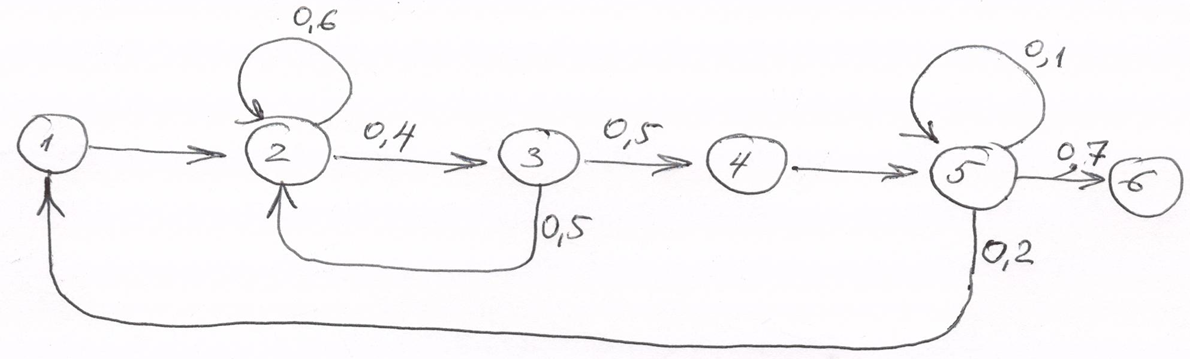
\includegraphics[width=.85\textwidth]{img/scheme_0}}
  \caption{Граф GERT-сети}
\end{figure}
\item Каждой дуге-работе ($ij$) поставлены в соответствие следующие данные:
\begin{enumerate}
\item Закон распределения времени выполнения работы. Будем считать его нормальным;
\item Параметры закона распределения (математическое ожидание \textbf{M} и дисперсия \textbf{D});
\item Вероятность $p_{ij}$ выполнения работы, показанная на графе.
\end{enumerate}
\end{enumerate}


\subsection{Задание}
\subsubsection{Часть 1}
Используя методику GERT, изложенную в книге «Методы анализа сетей»\\
Найти:
\begin{enumerate}
\item Вероятность выхода в завершающий узел графа (для всех вариантов узел 6);
\item Производящую функцию длительности процесса от начального узла  до завершающего узла;
\item Математическое ожидание длительности процесса от начального узла  до завершающего узла;
\item Дисперсию ожидание длительности процесса от начального узла  до завершающего узла;
\end{enumerate}
В отчете перечислить все петли всех порядков, обнаруженные на графе, выписать уравнение Мейсона, получить решение для $W_E(S)$ и найти требуемые параметры. Примерно так, как это сделано в примере на стр. 403–409 книги Филипса и Гарсиа «Методы анализа сетей»
\subsubsection{Часть 2}
Повторить пункты задания 2, 3, 4 используя методику анализа потокового графа, основанную на обработке матрицы передач (Branch Transmittance Matrix). 


Для выполнения задания рекомендуется пользоваться следующими источниками:
\begin{enumerate}
\item Филипс и Гарсиа «Методы анализа сетей»
\item Презентация GERT\_\&\_Flowgraph\_Algebra.pdf (выложена в ИНТРАНЕТ)
\item Ren\_The Methodology of Flowgraph.pdf
\end{enumerate}

\section{Решение}

\subsection{Часть 1}
Чтобы определить эквивалентную W-функцию для анализируемой GERT-сети, необходимо замкнуть сеть дугой, исходящей из узла 6 в узел 1 (рис. \ref{pic_1}).
\begin{figure}[H]
  \centering
  \fbox{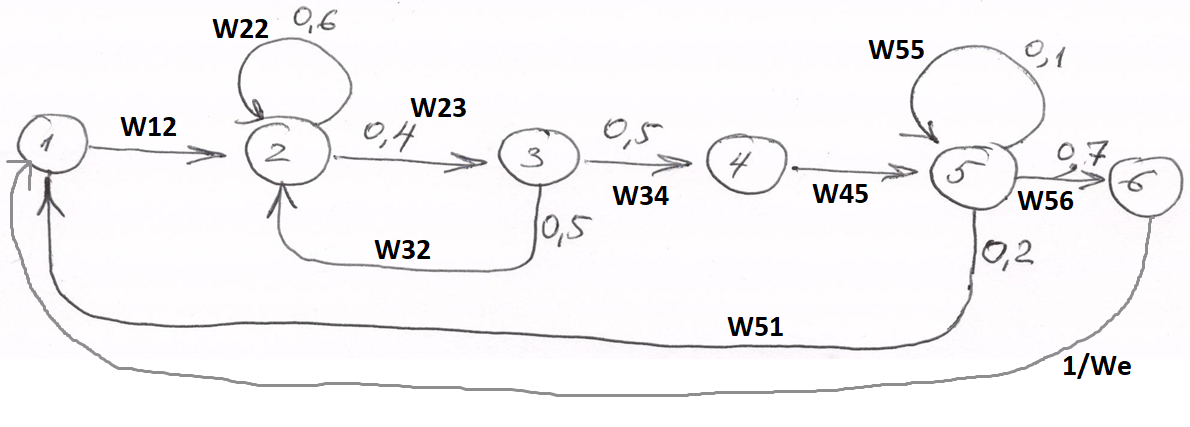
\includegraphics[width=\textwidth]{img/scheme_1}}
  \caption{Замкнутая GERT-сеть}
  \label{pic_1}
\end{figure}
Далее, выпишем в таблицу данные графа(мат. ожидание, дисперсия, W-функции)

\tabulinesep = 1mm
\begin{longtabu} to \textwidth {|X[8,c , m ] |X[8,c , m ] | X[15,l, m ]| X[15,l, m ]|X[15,l, m ]|X[25,l, m ]|}\firsthline\hline
\textbf{Начало}&\textbf{Конец}&\textbf{Вес ребра}&\textbf{Мат. ожидание}&\textbf{Дисперсия}&\textbf{W-функция}\\ \hline \endfirsthead
1	&2	&1	&20	&9	&$exp(20s+4.5s^2)$	\\ \hline
2	&2	&0.6&30	&16	&$0.6*exp(30s+8s^2)$	\\ \hline
2	&3	&0.4&40	&25	&$0.4*exp(40s+12.5s^2)$	\\ \hline
3	&2	&0.5&28	&16	&$0.5*exp(28s+8s^2)$	\\ \hline
3	&4	&0.5&37	&16	&$0.5*exp(37s+8s^2)$	\\ \hline
4	&5	&1	&30	&25	&$exp(30s+12.5s^2)$	\\ \hline
5	&1	&0.2&30	&16	&$0.2*exp(30s+8s^2)$	\\ \hline
5	&5	&0.1&10	&4	&$0.1*exp(10s+2s^2)$	\\ \hline
5	&6	&0.7&30	&16	&$0.7*exp(30s+8s^2)$	\\ \hline
\caption{Данные анализируемой GERT-сети}
\end{longtabu}
\textbf{Петли первого порядка:}
\begin{itemize}
\item $W_{12}W_{23}W_{34}W_{45}W_{51}$;
\item $W_{12}W_{23}W_{34}W_{45}W_{56}\frac{1}{W_e}$;
\item $W_{22}$;
\item $W_{23}W_{32}$;
\item $W_{55}$;
\end{itemize}
\textbf{Петли второго порядка:}
\begin{itemize}
\item $W_{22}W_{55}$;
\item $W_{55}W_{23}W_{32}$;
\end{itemize}
\textbf{Уравнение Мейсона}:
\begin{multline*}
H = 1 - W_{12}W_{23}W_{34}W_{45}W_{51} - W_{12}W_{23}W_{34}W_{45}W_{56}\frac{1}{W_e} - W_{22} - W_{23}W_{32} - W_{55}\\
 + W_{22}W_{55} + W_{55}W_{23}W_{32} = 0
\end{multline*}
\textbf{Выведем $W_E(S)$:}
\begin{equation*}
1 - W_{12}W_{23}W_{34}W_{45}W_{51} - W_{22} - W_{23}W_{32} - W_{55} + W_{22}W_{55} + W_{55}W_{23}W_{32} = W_{12}W_{23}W_{34}W_{45}W_{56}\frac{1}{W_e}
\end{equation*}
\begin{multline*}
W_E(S) =\\
(W_{12}W_{23}W_{34}W_{45}W_{56})/(1 - W_{12}W_{23}W_{34}W_{45}W_{51} - W_{22} - W_{23}W_{32} - W_{55} + W_{22}W_{55} + W_{55}W_{23}W_{32})
\end{multline*}

Вычислим математическое ожидание и дисперсию: $M_E(s) = 1$ при $s=0$

Так как $W_E(s)=p_E M_E (s)$,  то  $p_E=W_E(0)$, тогда $M_E(s)=\frac{W_E(s)}{p_E} =\frac{W_E(s)}{W_E(0)}$

Вычисляя первую и вторую производные по $s$ функции $M_E(s)$, и полагая $s=0$, находим математическое ожидание:
\begin{equation*}
\mu_{1E}=\frac{\partial M_E(s)}{\partial s}|s=0
\end{equation*}

и дисперсию:
\begin{equation*}
\sigma^2=\mu_{2E}-[\mu_{1E}]^2
\end{equation*}

Вероятность выхода в завершающий узел графа:
\begin{equation*}
p_E=W_E (0)
\end{equation*}
Для решения задачи был написан скрипт matlab, код приведен в приложении 4.

\begin{lstlisting}[language={matlab}, caption={Результат}, basicstyle=\ttfamily]
We =
-(7*exp((s*(91*s + 314))/2))/(5*exp(2*s*(s + 5)) - 3*exp(10*s*(s + 4)) + 30*exp(2*s*(4*s + 15)) - exp((3*s*(15*s + 52))/2) + 10*exp((s*(41*s + 136))/2) + 2*exp((s*(91*s + 314))/2) - 50)
 
We0 =
1
 
m1 =
2845/7
 
m2 =
11938987/49
 
D =
3844962/49
\end{lstlisting}
Были получены следующие результаты:
\begin{enumerate}
\item Вероятность выхода в завершающий узел графа равна 100\% ($p=W_E=1$).
\item Математическое ожидание 406,43.
\item Дисперсия времени выхода процесса в завершающий узел графа 78 468,61.
\end{enumerate}
\subsection{Часть 2}
Алгоритм дальнейших действий основан на:
\begin{itemize}
\item Презентация GERT\_\&\_Flowgraph\_Algebra.pdf (со слайда 56);
\item Ren\_The Methodology of Flowgraph.pdf (со страницы 35).
\end{itemize}
Определим матрицу Q, не забывая про обратную связь.
\begin{equation*}
Q = 
 \begin{pmatrix}
  0 & q_{12} & 0 & 0 & 0 & 0 \\
  0 & q_{22} & q_{23} & 0 & 0 & 0 \\ 
  0 & q_{32} & 0 & q_{34} & 0 & 0 \\ 
  0 & 0 & 0 & 0 & q_{45} & 0 \\ 
  q_{51} & 0 & 0 & 0 & q_{55} & q_{56} \\ 
  w_{61} & 0 & 0 & 0 & 0 & 0 
 \end{pmatrix}
\end{equation*}
Определим матрицу коэффициентов $A=I_6-Q^T$.
\begin{equation*}
A = 
 \begin{pmatrix}
    1&       0&    0&    0&    -q_{51}& -w_{61}\\
 -q_{12}& 1 - q_{22}& -q_{32}&    0&       0&    0\\
    0&    -q_{23}&    1&    0&       0&    0\\
    0&       0& -q_{34}&    1&       0&    0\\
    0&       0&    0& -q_{45}& 1 - q_{55}&    0\\
    0&       0&    0&    0&    -q_{56}&    1
 \end{pmatrix}
\end{equation*}
Находим 
\begin{equation*}
det(A)
\end{equation*}
далее
\begin{equation*}
\frac{\partial det(A)}{\partial w_{61}}
\end{equation*}
\begin{equation*}
det(A | w_{61}=0)
\end{equation*}
Далее можно вывести $W_E(S)$ с помощью формулы:
\begin{equation*}
W_E(S)=-\frac{\frac{\partial det(A)}{\partial w_{61}}}{det(A | w_{61}=0)}
\end{equation*}
Для расчетов, был написан matlab скрипт, код представлен в приложении 5.

\begin{lstlisting}[language={matlab}, caption={Результат}, basicstyle=\ttfamily]
[    1,       0,    0,    0,    -q51, -w61]
[ -q12, 1 - q22, -q32,    0,       0,    0]
[    0,    -q23,    1,    0,       0,    0]
[    0,       0, -q34,    1,       0,    0]
[    0,       0,    0, -q45, 1 - q55,    0]
[    0,       0,    0,    0,    -q56,    1]
 
 
-(q12*q23*q34*q45*q56)/(q22 + q55 + q23*q32 - q22*q55 - q23*q32*q55 + q12*q23*q34*q45*q51 - 1)
\end{lstlisting}
Во второй строчке был получен $W_E(S)$, который полностью(за исключением знаков) совпадает с $W_E(S)$ найденным в части 1.

Далее, имея $W_E(S)$ находим необходимые переменные.

Для расчетов, был использован скрипт из приложения 6.

\begin{lstlisting}[language={matlab}, caption={Результат}, basicstyle=\ttfamily]
We =
-(7*exp((s*(91*s + 314))/2))/(5*exp(2*s*(s + 5)) - 3*exp(10*s*(s + 4)) + 30*exp(2*s*(4*s + 15)) - exp((3*s*(15*s + 52))/2) + 10*exp((s*(41*s + 136))/2) + 2*exp((s*(91*s + 314))/2) - 50)
 
We0 =
1
 
m1 =
2845/7
 
m2 =
11938987/49
 
D =
3844962/49
\end{lstlisting}
Были получены следующие результаты:
\begin{enumerate}
\item Вероятность выхода в завершающий узел графа равна 100\% ($p=W_E=1$).
\item Математическое ожидание 406,43.
\item Дисперсия времени выхода процесса в завершающий узел графа 78 468,61.
\end{enumerate}
Которые полностью совпадает с результатами части 1. % Вариант 13

%------------------------------------------------------------------------------

\newpage
\section{Поиск оптимальной стратегии принятия решений с использованием марковских моделей.}

\subsection{Постановка задачи}
Пусть имеется машина (станок), которая обслуживается периодически один раз в час. В каждый момент она может находиться в одном из двух состояний: рабочем (состояние 1) и нерабочем (состояние 2).

Если машина на некотором шаге проработала непрерывно 1 час, то доход равен 3 рублям. При этом вероятность остаться на следующем шаге в состоянии 1 равна 0,7, а вероятность перейти в состояние 2 равна 0,3. Если машина отказала на некотором шаге, то её можно отремонтировать двумя способами. Первый является ускоренным, требует затрат в 2 рубля (доход равен -2 рубля) и обеспечивает переход в состояние 1 с вероятностью в 0,6. Второй, обычный способ требует затрат в 1 рубль и обеспечивает переход в состояние 1 с вероятностью 0,4.

Найти оптимальную стратегию для $N=\infty$ методом итераций по стратегиям, и перечислить все стационарные стратегии; построить марковскую модель принятия решений.

\subsection{Марковская модель принятия решений}

Матрицы переходных вероятностей ($P_1$ и $P_2$) и матрицы доходов ($r_1$ и $r_2$) имеют следующий вид:

\[ P_1 = \left( \begin{array}{cc}
0,7 & 0,3 \\
0,6 & 0,4
\end{array} \right)\qquad
%
P_2 = \left( \begin{array}{cc}
0,7 & 0,3 \\
0,4 & 0,6
\end{array} \right)
\]

\[ r_1 = \left( \begin{array}{rr}
3 & 0 \\
-2 & 0
\end{array} \right)\qquad
%
r_2 = \left( \begin{array}{rr}
3 & 0 \\
-1 & 0
\end{array} \right)
\]

Модель представлена на рисунке 3.

\begin{figure}[!h]
	\centering
	\begin{tikzpicture}[->,>=stealth',shorten >=1pt,auto,node distance=4cm,
	  thick,main node/.style={circle,fill=blue!20,draw,font=\sffamily\Large\bfseries}]

	  \node[main node] (1) {$S_1$};
	  \node[main node] (2) [below left of=1] {$D_1$};
	  \node[main node] (3) [below right of=2] {$S_2$};
	  \node[main node] (4) [below right of=1] {$D_2$};

	  \path[every node/.style={font=\sffamily\small}]
	    (1) edge node {0,3} (3)
	        edge [loop above] node {0,7} (1)
	    (2) edge [bend left] node [right] {0,6} (1)
	        edge node[right] {0,4} (3)
	    (3) edge [red, bend left] node [left] {2} (2)
	        edge [red, bend right] node[right] {1} (4)
	    (4) edge node [left] {0,6} (3)
	        edge [bend right] node[right] {0,4} (1);
	\end{tikzpicture}
	\caption{$S_1$ и $S_2$ состояния системы; $D_1$ и $D_2$ принимаемые решения; красные рёбра - траты, чёрные - вероятность перехода}
\end{figure}

После работы, машина можем:
\begin{itemize}
\item Остаться в исправном состоянии
$f^1 = \langle 1; 1 \rangle$
\item Перейти в неисправное состояние
$f^2 = \langle 1; 2 \rangle$
\end{itemize}

Таким образом, возможны следующие стационарные стратегии:
\begin{eqnarray*}
\pi_1^N = (f^1, f^1)\\
\pi_2^N = (f^1, f^2)\\
\pi_3^N = (f^2, f^1)\\
\pi_4^N = (f^2, f^2)
\end{eqnarray*}

\subsection{Метод итерации по стратегиям}

\textbf{Этап оценивания параметров}. Выбираем произвольную стратегию $\tau = (X_{j1}, X_{j2}, \dots, _{jm})^T$. Используя соответствующие стратегии $\tau$, матрицу переходных вероятностей $P(\tau) = (p_{ik}(\tau))$ и матрицу доходов $R(\tau) = (r_{jk}(\tau))$ и полагая $F_\tau(m) = 0$, решаем систему линейных алгебраических уравнений $E_\tau + F_\tau(j) - \sum\limits_{k=1}^m p_{jk}(\tau)F_\tau (k) = v_j (\tau)$, $j=\overline{1,m}$, относительно $E_\tau, F_\tau(1), \dots, F_\tau(m-1)$.

\textbf{Этап улучшения стратегии}. Для каждого состояния $S_j$, находим допустимое решение $X_{*j}$, на котором достигается $\text{max}_{(X_i \in G)}(v_j (X_i) + \sum\limits_{k=1}^m p_{jk}(X_i) F_\tau(k))$

Эти оптимальные решения образуют новую стратегию $t = (X_{*1}, X_{*2}, … X_{*m})^T$. Если $t = \tau$, то стратегия $\tau$ и является оптимальной. В противном случае нужно обозначить стратегию t через $\tau$ и вернуться к первому этапу.

Воспользовавшись матрицами $P_1$, $P_2$, $r_1$, $r_2$ и их независимостью от номера этапа, вычислим ожидаемые доходы, при различных вариантах допустимых решений:

\begin{eqnarray*}
v_1 (X_1 )=0,7*3 + 0,3*0=2,1		\\
v_2 (X_1 )=0,6*(-2) + 0,4*0=-1,2	\\
v_1 (X_2 )=0,7*3 + 0,3*0=2,1		\\
v_2 (X_2 )=0,4*(-1) + 0,6*0=-0,4
\end{eqnarray*}

В качестве произвольной стратегии $\tau$ используем стратегию номер два. В этом случае на этапе оценивания параметров, учитывая, что $F_\tau(2)=0$, получаем систему линейных алгебраических уравнений

$$
\left\{
	\begin{aligned}
	E_\tau + (1 - 0,7) F_\tau(1) &= & 2,1\\
	E_\tau - 0,6 &= & -1,2\\
	\end{aligned}
\right.
$$

которая имеет единственное решение: $E_\tau = 0,78$, $F_\tau(1) = 3,3$.

Результаты соответствующих вычислений приведены в табл. 5.

\begin{table}[htb]
	\begin{tabularx}{\textwidth}{|c|X|X|c|c|}
	\hline
	\multirow{2}{*}{$S_j$} & \multicolumn{2}{c|}{$\varphi (X_i )=v_j (X_k )+p_j1 (X_i)*F_i (1)$} & \multirow{2}{*}{max $\varphi_j$} & \multirow{2}{*}{$X_{*j}$} \\ 
	\hhline{~--~~}
	{} & i = 1 & i = 2 & {} & {} \\ 
	\hline 
	1 & 2,1+0,7*3,3=4,41 & 2,1+0,7*3,3=4,41 & 4,41 & $X_2$ \\ 
	\hline 
	2 & -1,2+0,6*3,3=0,78 & -0,4+0,4*3,3=0,92 & 0,78 & $X_2$ \\ 
	\hline
	\end{tabularx}
\caption{Решение с оценочными параметрами}
\end{table}

Новая стратегия $t = (X_2, X_2)^T$ отличается от стратегии $\tau$, поэтому нужно на этап оценивания параметров, полагая $\tau = (X_2, X_1)^T$.

Новой стратегии t соответствует следующая система линейных алгебраических уравнений:
$$
\left\{
	\begin{aligned}
	E_\tau + (1 - 0,7) F_\tau(1) &= & 2,1\\
	E_\tau - 0,4 &= & -0,4\\
	\end{aligned}
\right.
$$

которая имеет единственное решение: $E_\tau = 0,85$, $F_\tau(1) = 3,125$.

Результаты соответствующих вычислений приведены в табл. 6.

\begin{table}[htb]
	\begin{tabularx}{\textwidth}{|c|X|X|c|c|}
	\hline
	\multirow{2}{*}{$S_j$} & \multicolumn{2}{c|}{$\varphi (X_i )=v_j (X_k )+p_j1 (X_i)*F_i (1)$} & \multirow{2}{*}{max $\varphi_j$} & \multirow{2}{*}{$X_{*j}$} \\ 
	\hhline{~--~~}
	{} & i = 1 & i = 2 & {} & {} \\
	\hline
	1 & 2,1+0,7*3,125=4,2875 & 2,1+0,7*3,125=4,2875 & 4,2875 & $X_2$ \\
	\hline
	2 & -1,2+0,6*3,125=0,675 & -0,4+0,4*3,125=0,85 & 0,85 & $X_2$ \\
	\hline
	\end{tabularx}
\caption{Проверочное решение}
\end{table}

Новая стратегия совпала с предыдущей, таким образом оптимальная стратегия определена: оптимальное использовать более дешевый ремонт с меньшей гарантией успешного завершения.

\subsection{Метод линейного программирования}

Все параметры посчитаны, мы можем сформулировать задачу в виде задачи линейного программирования, для проверки ранее полученных результатов.

$$
\left\{
	\begin{aligned}
	2,1w_{11}+2,1w_{12}-1,2w_{21}-0,4w_{22} & ->& \text{max}\\
	0,3w_{11}+0,3w_{12}-0,6w_{21}-0,4w_{22} & = & 0 \\
	-0,3w_{11}-0.3w_{12}+0,6w_{21}+0,4w_{22} & = & 0 \\
	\sum\limits_{j=1}^2 \sum\limits_{i=1}^2 w_{ij}=1,\qquad w_{ij} \geq 0 &&\\
	\end{aligned}
\right.
$$

Код скрипта представлен в листинге 9.

\lstinputlisting[language=Matlab, caption={Код для вычисления задачи линейного программирования}]{../task3/linear.m}

\newpage

Результат выполнения в листинге 10.

\lstinputlisting[language={},caption={Результат работы скрипта линейного программирования}]{../task3/linear.out}

Таким образом, оптимальной стратегии снова стало использование дешевого ремонта, как и в предыдущем случае с итерации по стратегиям. % Вариант 26, стр 273

%------------------------------------------------------------------------------

\newpage
\section{Поиск оптимальных параметров сети систем массового обслуживания.}

\subsection{Постановка задачи}
Минимизировать стоимость ССМО при ограничении на среднее число заявок в сети

\begin{gather*}
min\{F(u) = \sum\limits_{j=1}^n \sum\limits_{k=1}^{n_j} f_{jk} u_{jk} = \sum\limits_{j=1}^n \sum\limits_{k=1}^{n_j} (m_{jk} * \mu_{jk}) * u_{jk} \}
\end{gather*} 

$ L(u) = \sum\limits_{j=1}^n L_{jk} u_{jk}$,

$ u_{jk} =
  \begin{cases}
    0,\\
    1
 \end{cases}$,
 
Дано многоканальная сеть Джексона:

\begin{gather*}
\{ \lambda_0, \{jk\} - \text{набор альтернатив}, Q=\{q_{ij}\}_{i=\overline{0,n}, j=\overline{0,n}}, L(u) \}
\end{gather*} 

$L(u) = 4$, (предельное число заявок в сети)

$\lambda_0 = 6$,

$Q=\{q_{ij}\}_{i=\overline{0,n}, j=\overline{0,n}} = \begin{tabular}{|c|c|c|c|c|}
\hline 
0 & 0,2 & 0,7 & 0 & 0,1 \\ 
\hline 
0,1 & 0 & 0,1 & 0,2 & 0,6 \\ 
\hline 
0,5 & 0,1 & 0 & 0,2 & 0,2 \\ 
\hline 
0 & 0,2 & 0,8 & 0 & 0 \\ 
\hline 
0,3 & 0,2 & 0,2 & 0,3 & 0 \\ 
\hline 
\end{tabular} $.

Самостоятельно сформировать набор альтернатив (по 2 альтернативы на каждый узел, обеспечивающих установивший режим в узле).

Решить задачу 5 двумя способами:

\begin{itemize}
\item В соответствии с алгоритмом 5
\item Как задачу дискретного линейного программирования (например, с использованием Матлабовской команды Linprog).
\end{itemize}

\subsection{Алгоритм решения}

\begin{enumerate}
	\item Найти $\lambda_i, j = 1. \dots, m$ -- скорость прихода задач в узел $j$.\\
	$\lambda_{ij}=\lambda_i q_{ij}$	
	$\lambda_j = \lambda_{0j} + \sum\limits_{i=1}^n q_{ij}\lambda_i$, при $j=1,\dots,n$\\
	\item Возьмем произвольный набор альтернатив для каждого узла.\\
	$[(m_j^1,\mu_j^1),(m_j^1,\mu_j^1),\dots,(m_j^k,\mu_j^k)]$
	\item $p_j$ рассчитывается по следующей формуле\\
	$p_j = \frac{\lambda_j}{\mu_j m_j}$
	\item Вычислим $E(W_{qj})$:\\
	$E(W_{qj}) = \frac{(m_j p_j)^{m_j} \pi(0)}{\mu_j m_j (1-p_j)^2 m_j!}$, где
	$\pi(0) = \{\sum\limits_{t=0}^{m_j - 1} \frac{(m_j p_j)^t}{t!} + \frac{(m_j p_j) ^ m_j}{(1-p_j)m_j!}  \}^{-1}$
	\item Найдем $L_j$ -- число заявок в j-ом узле по формуле:\\
	$L_j = [E(W_{qj} + E(S_j)] \lambda_i$, где $E(S_j)= \frac{1}{\mu}$
\end{enumerate}

\subsection{Решение по алгоритму}

\textbf{Первый шаг алгоритма}

По первой формуле из первого шага алгоритма найдем вектор $\lambda_{0j}$.\\
$\lambda_{0j}= (1,2 \qquad 4,2 \qquad 0 \qquad 0,6)$

Используя вектор $\lambda_{0j}$, составим систему уравнений по второй формуле из шага 1.

$$
\left\{
	\begin{aligned}
	\lambda_0 &= & 6\\
	\lambda_1 &= & 1,2 + 0,2 * \lambda_0 +0,1 * \lambda_2 + 0,2 * \lambda_3 + 0,2 * \lambda_4\\
	\lambda_2 &= & 4,2 + 0,7* \lambda_0 + 0,1 * \lambda_1 +0,8 * \lambda_3 +0,2 * \lambda_4\\
	\lambda_3 &= & 0,2 * \lambda_1 +0,2 * \lambda_2 +0,3  * \lambda_4\\
	\lambda_4 &= & 0,6 + 0,1 * \lambda_0 + 0,6 * \lambda_1 + 0,2 * \lambda_2\\
	\end{aligned}
\right.
$$

В результате решения системы методом Гаусса был получен следующий результат:
\begin{itemize}
\item $\lambda_0 = 6 $;
\item $\lambda_1 = 7,44 $;
\item $\lambda_2 = 17,06 $;
\item $\lambda_3 = 7,63 $;
\item $\lambda_4 = 37,65 $.
\end{itemize}

Теперь вычислим остальные $\lambda_{ij}$, используя следующий скрипт. Здесь и в дальнейшем используется странное ограничение на предельное число заявок в сети -- 4 шт. вместе с нулевой.

\begin{Verbatim}[frame=single]
% Исходные данные
Q = [0 0.2 0.7 0 0.1;
    0.1 0 0.1 0.2 0.6;
    0.5 0.1 0 0.2 0.2;
    0 0.2 0.8 0 0;
    0.3 0.2 0.2 0.3 0];
% Значение лямбды каждого узла
lambdaj=[6;7.44;17.06;7.63;37.65];
N=4; % Число узлов вместе с нулевой.
% Вычисление лямбда ij
lambdaij=[];
 for i = 1:N
    for j = 1:N
         lambdaij(i,j) = lambdaj(i)*Q(i, j);
    end
end
lambdaij
\end{Verbatim}

Результаты вычисления представлены в таблице 7.

\begin{table}[htb]
	\begin{tabularx}{\textwidth}{|c|X|X|X|X|}
	\hline 
	i\textbackslash{}j & 1 & 2 & 3 & 4 \\ 
	\hline 
	1 &  0 & 1.2000 & 4.2000 & 0 \\ 
	\hline 
	2 & 0.7440 & 0 & 0.7440 & 1.4880 \\ 
	\hline
	3 & 8.5300 & 1.7060 & 0 & 3.4120 \\ 
	\hline 
	4 & 0 & 1.5260 & 6.1040 & 0 \\ 
	\hline 
	\end{tabularx}
\caption{Результат вычисления всех значений $\lambda_{ij}$}
\end{table}

\textbf{Второй шаг алгоритма}

Далее сформируем набор альтернатив (по 2 альтернативы на каждый узел, обеспечивающих установивший режим в узле):
\begin{itemize}
\item $m_j^1$=(4 8 3 4);
\item $\mu_j^1$=(2 3 7 9);
\item $m_j^2$=(5 8 3 6);
\item $\mu_j^2$=(9 13 10 4);
\end{itemize}

\textbf{Третий шаг алгоритма}

Для расчета вероятности $p_j$ воспользуемся следующим скриптом:
\begin{Verbatim}[frame=single]
K=2; % Задаем альтернативы
muj = [4 8 3 4;
       2 3 7 9];
 
mj = [5 8 3 6;
      9 13 10 4];

% Расчёт вероятностей
pj = [];
 for i = 1:N-1
    for k = 1:K
        pj(k,i) = lambdaj(i+1)/(muj(k,i)*mj(k,i));
    end
 end
pj
\end{Verbatim}

Результаты занесены в таблицу 8.

\begin{table}[htb]
	\begin{tabularx}{\textwidth}{|c|X|X|X|}
	\hline 
	k\textbackslash{}j & 1 & 2 & 3 \\ 
	\hline 
	1 & 0.3720 & 0.2666 & 0.8478 \\
	\hline 
	2 & 0.4133 & 0.4374 & 0.1090 \\
	\hline 
	\end{tabularx}
\caption{Результат расчёта вероятностей}
\end{table}

\textbf{Четвертый шаг алгоритма}

Расчет вектора $\pi_j (0)$.

\begin{Verbatim}[frame=single]
% Расчет начальной вероятности для каждого узла.
pij0 = [];
for i = 1:N-1
    for k=1:K
        sum = 0;
        for t = 0:mj(k,i)-1
            sum = sum + ((mj(k,i)*pj(k,i))^t)/factorial(t);
        end
        sum = sum + ((mj(k,i)*pj(k,i))^mj(k,i))/
                                    ((1-pj(k,i))*factorial(mj(k,i)));
        pij0(k,i)=sum^(-1);
    end
end
pij0
\end{Verbatim}

Результаты расчета начальной вероятности узлов занесены в таблицу 9.

\begin{table}[htb]
	\begin{tabularx}{\textwidth}{|c|X|X|X|}
	\hline 
	k\textbackslash{}j & 1 & 2 & 3 \\ 
	\hline 
	1 & 0.1549 & 0.1185 & 0.0403 \\ 
	\hline 
	2 & 0.0242 & 0.0034 & 0.3362 \\ 
	\hline 
	\end{tabularx}
\caption{Расчет начальной вероятности узлов}
\end{table}

\textbf{Пятый шаг алгоритма}

Рассчитаем $E(W_{q_j})$.

\begin{Verbatim}[frame=single]
% E(Wqj) для каждого узла.
EWqj = [];
for i = 1:N-1
    for k=1:K
        EWqj(k,i) = (((mj(k,i)*pj(k,i))^mj(k,i))*pij0(k,i))/
        	(muj(k,i)*mj(k,i)*((1-pj(k,i))^2)*factorial(mj(k,i)));
    end
end     
EWqj
\end{Verbatim}

Результаты занесены в таблицу 10.

\begin{table}[htb]
	\begin{tabularx}{\textwidth}{|c|X|X|X|}
	\hline 
	k\textbackslash{}j & 1 & 2 & 3 \\ 
	\hline
	1 & 0.0036 & 0.0000 & 0.5304 \\ 
	\hline 
	2 & 0.0015 & 0.0003 & 0.0000 \\ 
	\hline 
	\end{tabularx}
\caption{Расчет вектора $E(W_{q_j})$  для k=1 и k=2}
\end{table}

Теперь найдем $E(S_j)$ для каждого узла.
\begin{Verbatim}[frame=single]
% Найдем E(sj) для каждого узла.
Esj = [];
for i = 1:N-1
    for k=1:K
        Esj(k,i) = 1/muj(k,i);
    end
end  
Esj
\end{Verbatim}

Результаты занесены в таблицу 11.

\begin{table}[htb]
	\begin{tabularx}{\textwidth}{|c|X|X|X|}
	\hline 
	k\textbackslash{}j & 1 & 2 & 3 \\ 
	\hline 
	1 & 0.2500 & 0.1250 & 0.3333 \\ 
	\hline 
	2 & 0.5000 & 0.3333 & 0.1429 \\ 
	\hline 
	\end{tabularx}
\caption{Расчет $E(S_j)$ для каждого узла.}
\end{table}

Теперь не составит труда посчитать $L_j$ --  число заявок в j-ом узле, для каждой альтернативы.

\begin{Verbatim}[frame=single]
% Найдем Lj
Lj = [];
for i = 1:N-1
    for k=1:K
        Lj(k,i) = lambdaj(i+1)*(EWqj(k,i)+Esj(k,i));
    end
end
Lj
\end{Verbatim}

Результаты занесены в таблицу 12.

\begin{table}[htb]
	\begin{tabularx}{\textwidth}{|c|X|X|X|}
	\hline 
	k\textbackslash{}j & 1 & 2 & 3 \\ 
	\hline 
	1 & 1.8871 & 2.1331 & 6.5900 \\ 
	\hline 
	2 & 3.7309 & 5.6916 & 1.0900 \\ 
	\hline 
	\end{tabularx}
\caption{Расчет числа заявок в каждом узле.}
\end{table}

Таким образом, сеть не загружена и простаивает.

\subsection{Решение дискретным линейным методом программирования}

Для решения задачи воспользуемся функцией bintprog.

\begin{Verbatim}[frame=single]
%Зададим входные параметры
A = [1 0 0 1 0 0;
     0 1 0 0 1 0;
     0 0 1 0 0 1];
f = [4 4 5 5 2 31];
b = [1 1 1];
Aeq = A;
beq = [1;1;1];
[x, fval] = bintprog(f,A,b,Aeq,beq)
%параметры A,b,Aeq,beq будут как для прошлой задачи
%дополнительно введем ограничения на значение lb и ub
lb=zeros(1,(N-1)*2);
ub=ones(1,(N-1)*2);
%решаем задачу
[x,fval] = linprog(f,A,b,Aeq,beq,lb,ub)
\end{Verbatim}

Результаты представлены в таблице 13.

\begin{table}[htb]
	\begin{tabularx}{\textwidth}{|c|X|X|X|}
	\hline 
	k & $u_{1k}$ & $u_{2k}$ & $u_{3k}$ \\ 
	\hline 
	1 & 1 & 1 & 1 \\ 
	\hline 
	2 & 0 & 0 & 0 \\ 
	\hline 
	\end{tabularx}
\caption{Результат использования linprog.}
\end{table}

Получаем следующий выбор альтернатив: ($u_{11}$, $u_{21}$, $u_{31}$).
 % Вариант 154, задача 5

%------------------------------------------------------------------------------

%\input{literature}
\newpage
\section*{Список используемой литературы}
\addcontentsline{toc}{section}{Список используемой литературы}

1.	Колесников Д.Н., Бендерская Е.Н., Лупин А.В., Пахомова В.И., Сиднев А.Г., Цыган В.Н. «Системный анализ и принятие решений». СПб.: Издательство Политехнический университет, 2008. - 468с.

2.	Макаров И.М., и др. Теория выбора и принятия решений. М. Наука. 1982. — 328 с.

3.	Вишневский В.М. «Теоретические основы проектирования компьютерных сетей». — М. : Техносфера, 2003. - 512 с

%------------------------------------------------------------------------------

\end{document}